\documentclass{article}
%packages
\usepackage{graphicx}
\usepackage[utf8]{inputenc}
\usepackage[T1]{fontenc}
\usepackage[frenchb]{babel}
\usepackage[a4paper]{geometry}
\usepackage{minted}
\usepackage{hyperref}
\usepackage[final]{pdfpages}

\begin{document}
%title
\begin{titlepage}
	\vspace{-20px}
	\begin{tabular}{l}
		
\includegraphics[scale=0.1]{esir.png}\\
		\\
		\textsc{Blin} S\'ebastien\\
		ESIR 1 - Informatique\\
		2014-2015\\
		\\
		\textsc{Engel} Jean-Christophe\\
		Maître de conférences à l'ESIR
	\end{tabular}
	\hfill
	\begin{tabular}{l}
		
\includegraphics[scale=0.5]{telecom}\\
		Télécom Bretagne\\
		2 Rue de la Châtaigneraie,\\
		35510 Cesson-Sévigné\\
		+33 2 99 12 70 00\\
		\\
		\textsc{Toutain} Laurent\\
		Maître de conférences\\
		Département RSM
	\end{tabular}
	\vfill
	\begin{center}
		\vspace{0.5cm}\hrule\vspace{0.5cm}
		\LARGE{\textbf{Rapport de stage}}\\
		\Large{Télécom Bretagne - Projet LoRa FABian}
		\vspace{0.5cm}\hrule
	\end{center}
	\vfill
	\begin{flushleft}
		\Large{Année universitaire 2014-2015}
		\hspace{4cm}
		
\includegraphics[scale=0.6]{univ}
	\end{flushleft}
\end{titlepage}
%%%%%%%%%%%%%%%%%%%%%%%%%%%%%%%%%%%%%%%%%%%%%%%%%%%%%%%%%%%%%%%%%%%%%%%%%%%%%%%%%%%%%%%%%%%%%%%%%%%%%%%%%%%%
\begin{titlepage}
\textbf{Remerciements}
\newline\newline
Je tiens à remercier toutes les personnes qui ont contribué au succès de mon stage et qui m'ont aidé lors de la rédaction de ce rapport.
\newline\newline
Tout d'abord, je tiens à remercier mon maître de stage Mr Laurent \textsc{Toutain} - Maître de conférences à Télécom Bretagne et Mr Alexander \textsc{Pelov} - Maître de conférences dans le département RSM (Réseaux, Sécurité, Multimédia) de Télécom Bretagne pour m'avoir accueilli en stage et leur partage d'expertise ainsi que pour les missions intéressantes que j'ai eu la possibilité de réaliser.
\newline\newline
Je remercie aussi le département RSM de Télécom Bretagne et plus particulièrement Mathieu \textsc{Goessens}, Tanguy \textsc{Kedoncuff}, Renzo \textsc{Navas} et Sarah \textsc{Tarrapey} pour leur temps donné, leur confiance et leurs explications qui m'ont été d'une grande aide tout au long de la durée de mon stage.
\newline\newline
Enfin, je remercie Marie-Pierre \textsc{Yvenat} pour le suivi administratif fournit.
\end{titlepage}

\thispagestyle{empty}
\tableofcontents
\listoffigures
\newpage
\setcounter{page}{1}

%%%%%%%%%%%%%%%%%%%%%%%%%%%%%%%%%%%%%%%%%%%%%%%%%%%%%%%%%%%%%%%%%%%%%%%%%%%%%%%%%%%%%%%%%%%%%%%%%%%%%%%%%%%%
\section{Introduction}
\subsection{Télécom Bretagne}
Télécom Bretagne est une école d'ingénieurs généraliste et un centre de recherche international en sciences et technologies de l'information et membre fondateur de l'Université Européenne de Bretagne. L'école fait aussi partie de l'Institut Mines-Télécom. La structure fut créée en 1977 et possède aujourd'hui des campus à Brest, Rennes, Toulouse. L'école compte 70\% d'élèves Ingénieurs et 30\% d'élèves en 3e cycle (dont 200 doctorants).\\
Télécom Bretagne est actif dans quatre pôles de compétitivité (Images et Réseaux, Mer Bretagne, ID4Car et Valorial). Les projets de recherche sont répartis dans quatre différents laboratoires, dont deux au CNRS (Labstic et Irisa), un à l'Inserm et un laboratoire Marsouin. Cette recherche est centrée sur les STIC dans différents champs d'application (Santé, Mer, Défense, Finances, Banques, Transports, etc).\\
Plus précisément, le département « Réseaux, Sécurité et Multimédia » (RSM) dans lequel ce stage c'est déroulé est composé de 60 personnes (17 permanents, des CDD, des thésards et des stagiaires). Ce département voit son activité accès autour de la recherche sur les réseaux, (IPv6, réseaux mobiles, sécurité des réseaux ou Internet des Objets). Mon stage c'est déroulé dans l'équipe OCIF (Objets communicants pour l'Internet du Futur) qui a pour but de définir, d’évaluer et de valider les architectures protocolaires liées à l’Internet des Objets.
\subsection{Objectifs personnels}
Ce stage était pour moi une occasion de découvrir en quoi consistait le travail sur un projet en tant qu'ingénieur de recherche dans un laboratoire. De plus, j'ai pu découvrir quelques problématiques d'un projet d'entreprise dans l'open-source (notamment la question de la licence de publication des morceaux de codes et les choix technologiques) et de découvrir le monde du travail dans le domaine de l'embarqué (hésitant actuellement entre une professionnalisation dans l'embarqué ou dans l'apprentissage automatique (Machine Learning) en dernière année).

\section{Mission au sein de Télécom Bretagne}
Le projet LoRa FABian est un projet visant à offrir des technologies libres et standardisées pour les besoins des objets communicants (IoT - Internet of Things). Construit autour de protocoles longue portée LoRa de Semtech\footnote{\url{http://www.semtech.com/wireless-rf/lora.html}} et CoAP\footnote{version simplifiée d'HTTP, initialement prévue pour fonctionner au-dessus d'UDP - The Constrained Application Protocol - \url{https://tools.ietf.org/html/rfc7252}}, celui-ci prototype rapidement des services utilisant cette radio. Bien que 6LoWPAN\footnote{\url{https://www.ti.com/lsds/ti/wireless_connectivity/6lowpan/overview.page}} réduit l’impact du protocole IPv6 et associés, les contraintes de la radio poussent à utiliser directement le protocole CoAP sur LoRa avec un tramage compatible avec la norme IEEE 802.15.4. Le plan de signalisation (messages beacon\footnote{de signalisation}, enregistrement des noeuds) repose également sur ce protocole. À l'inverse d'autres solutions utilisant LoRa, l'approche de Télécom Bretagne repose sur des technologies ouvertes, standardisées et ambitionne d'être lui-même standardisé auprès de l'IETF\footnote{Internet Engeenering Task Force, le groupe de standardisation produisant les RFC}. Techniquement LoRa FABian repose sur une architecture multi-tiers, inspirée des réseaux 3G et 4G. Les objets connectés (aussi appelés noeuds F) communiquent via ondes radio à des fréquences en dessous du Ghz, sur de longues portées (plusieurs kilomètres), auprès d'antennes (noeuds R). Ces noeuds R sont eux-mêmes reliés à des noeuds G (concentrateurs/gateway) fournissant des services (comme l'authentification) auprès de noeuds dédiés (noeuds S/AAA). La communication entre les noeuds G et S se fait via HTTPS.\\

L'objectif de ce stage consiste à améliorer les implémentations existantes des noeuds F, construites autour d'Arduino et de shields produits par la société Wi6labs, dans le but de proposer une implémentation ouverte, documentée, facile à prendre en main. Le stage commencera par une découverte des protocoles impliqués, de l'architecture globale, des implémentations utilisées telles que l'OS Contiki et l'environnement Arduino. Il s’agira ensuite de développer les bibliothèques nécessaires à la communication entre les cartes Arduino et Wi6Labs et de les utiliser.\\

Le projet LoRa FABian est conduit en partenariat entre plusieurs entités~: Télécom Bretagne pour la conception protocolaire, Wi6labs pour la réalisation des shields, Kerlink pour la réalisation des antennes et l'AFNIC comme expert technique pour les problématiques liées au nommage et à la sécurité (DNS, DNSSEC, etc.).\\
Dans ce rapport, nous allons tout d'abord voir quels ont été les outils pris en main, puis comment est architecturé le projet LoRa FABian et enfin le déroulement de ma mission principale et les missions annexes.

\section{Travail effectué}
\subsection{Découverte des outils}

	\begin{figure}[h]
		\begin{center}
			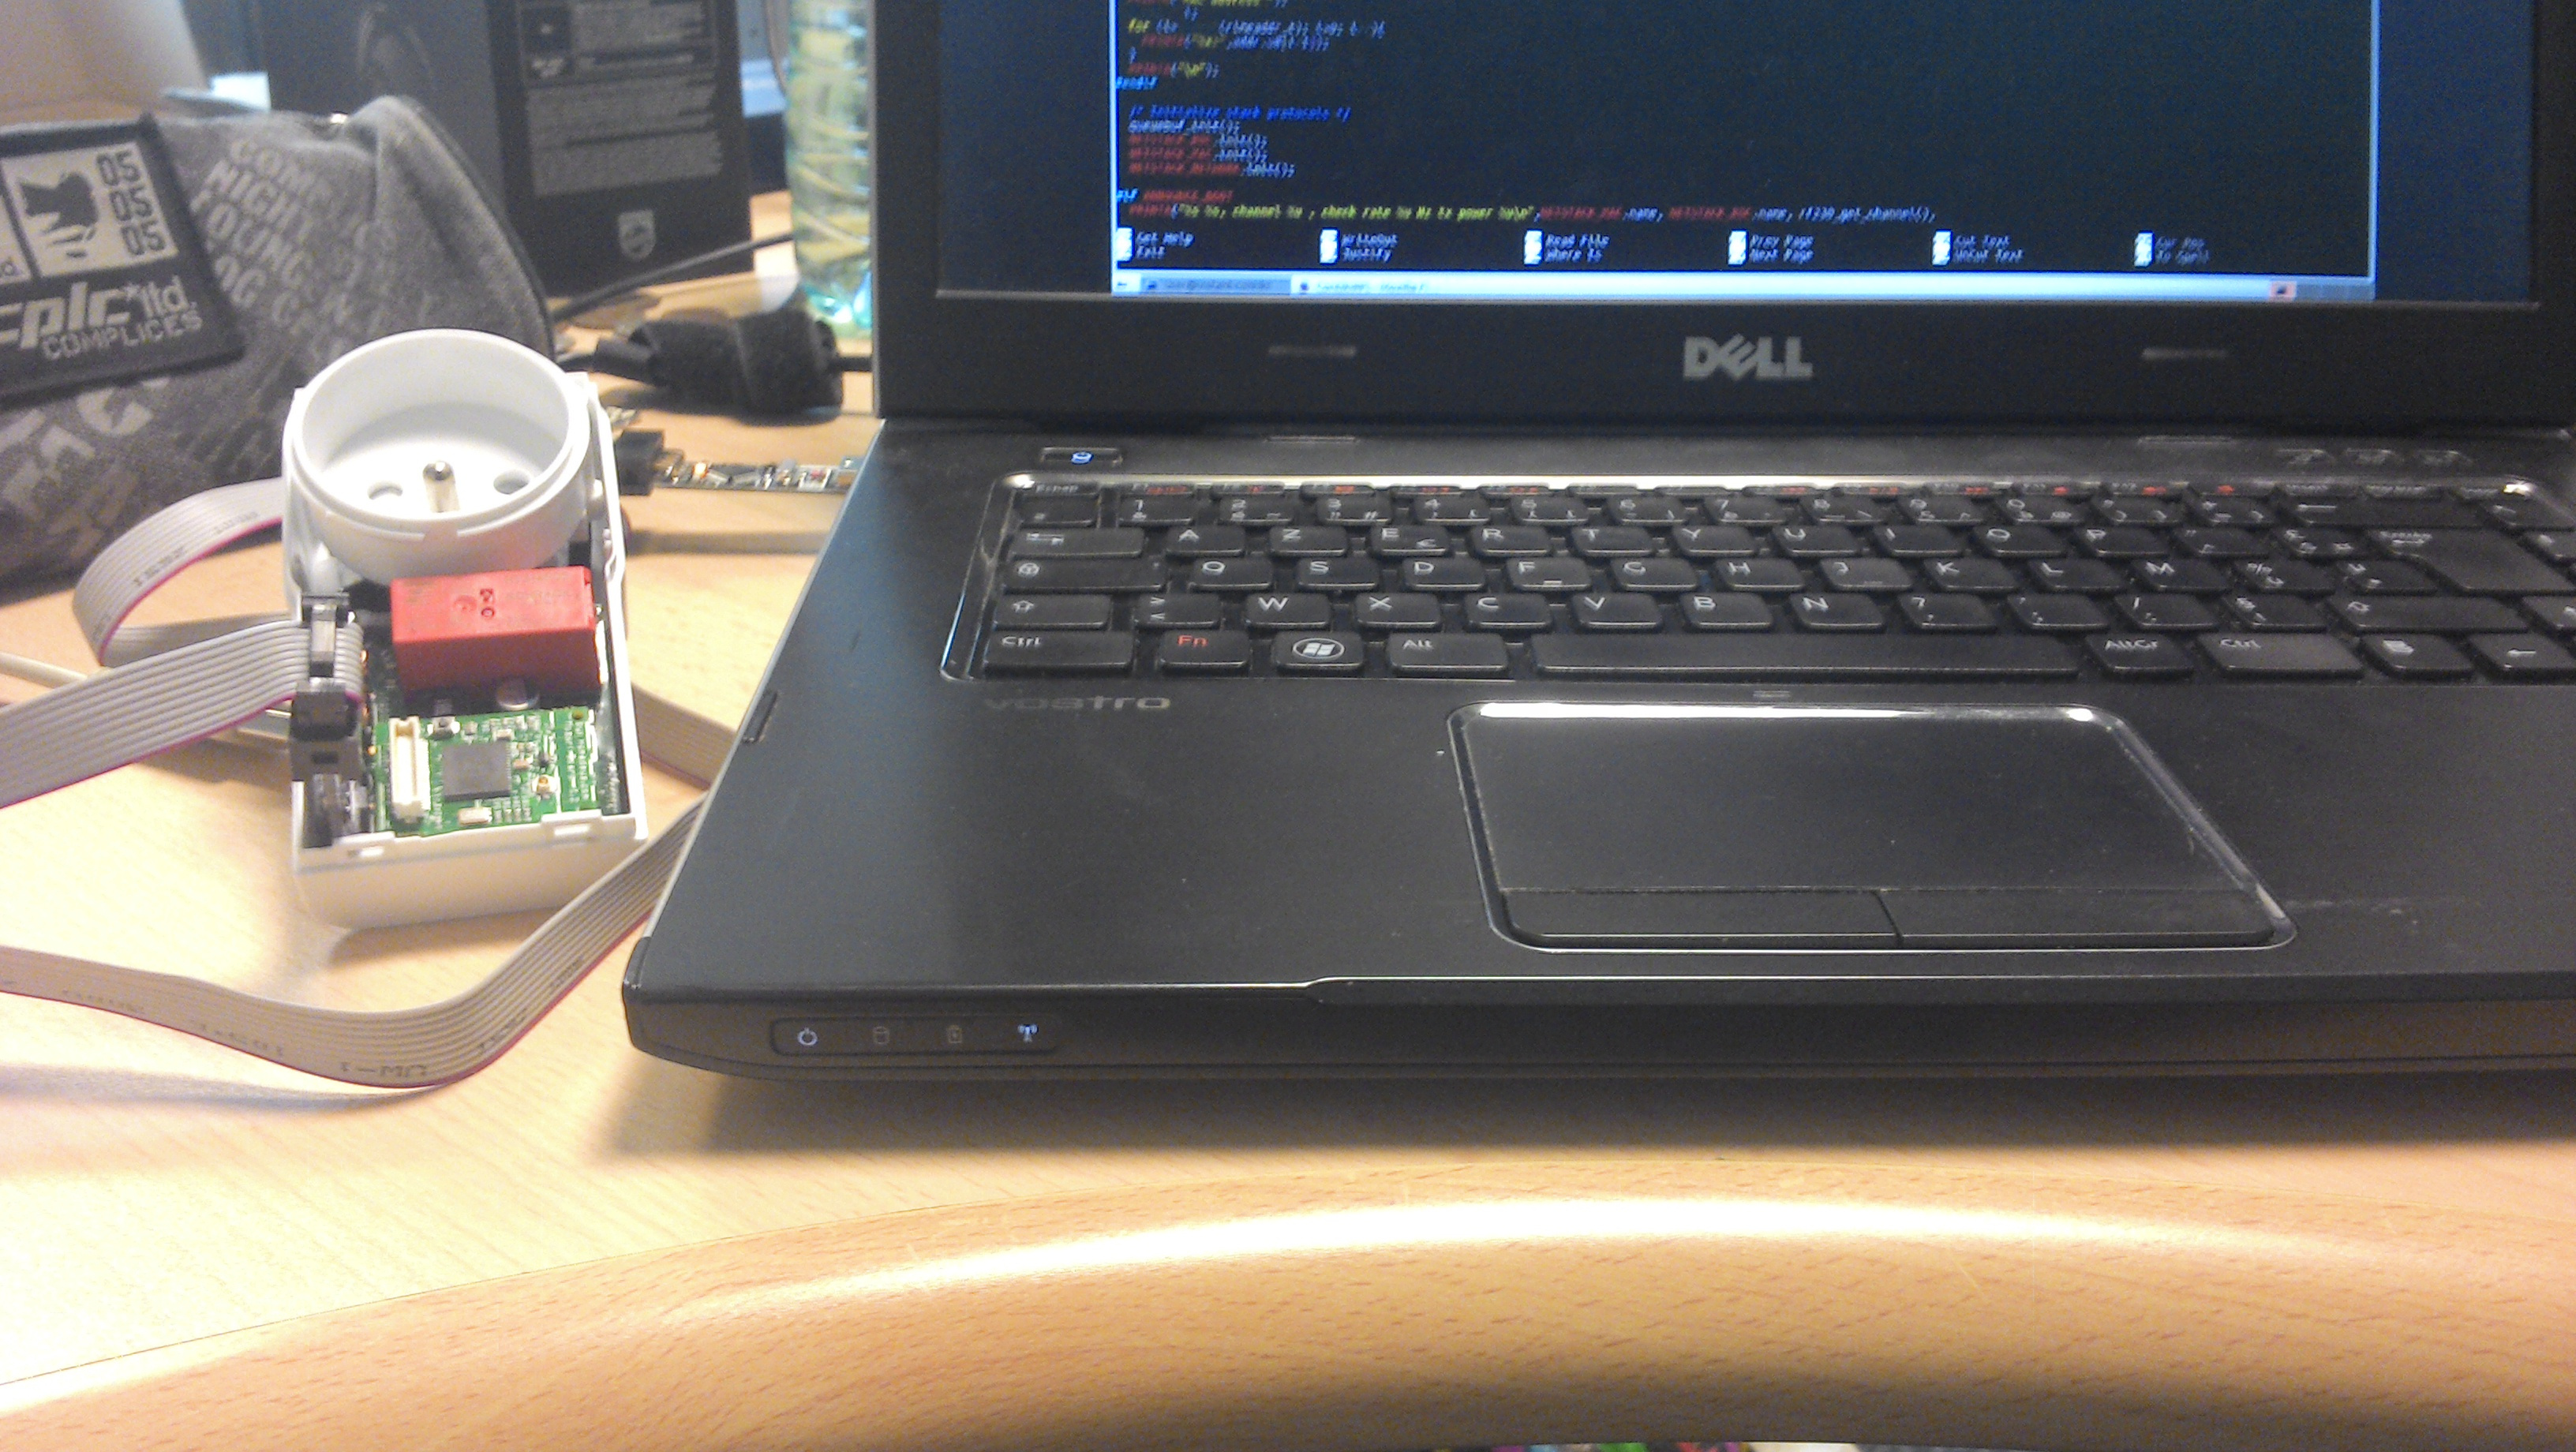
\includegraphics[scale=0.08]{../res/img/progprise.jpg}
			\caption{Programmation d'une prise sous Contiki OS}
			\label{fig:progprise}
		\end{center}
	\end{figure}

La première partie du stage consistait à la prise en main des différents outils qui ont été utilisés par la suite.\\
Concrètement, cette découverte fut réalisée en aidant à la réalisation de deux différents TPs (cf annexe C) pour un cours d'été.\\
Le premier TP consistait à contrôler des prises électriques par radio grâce à une puce embarquant le système d'exploitation Contiki via l'envoi de requêtes CoAP (envoyés via un script Python ou Bash ou l'extension Firefox Copper\footnote{\url{https://addons.mozilla.org/en-US/firefox/addon/copper-270430/}}). J'ai donc été amené à reprogrammer les cartes des prises électriques [Figure~: \ref{fig:progprise}] afin de les configurer, prendre en main la machine virtuelle fournie pour développer sur Contiki\footnote{\url{http://contiki-os.org/}} (à l'aide d'Instant Contiki) qui est une machine Ubuntu Linux avec les outils spécifiques à Contiki (Pour lister les appareils, les reprogrammer, etc.) et réaliser un script Python pour obtenir l'état d'une lampe ainsi qu'allumer une autre lampe.\\
Le second TP consistait à prendre en main le shield Arduino de la société Wi6labs fonctionnant aussi à l'aide d'un environnement Contiki afin de rendre le code Arduino plus lisible. J'ai aussi complété le code actuel pour pouvoir afficher une petite page web, allumer une led, etc. La configuration de la carte se faisait en modifiant la configuration de la partie Contiki et en reprogrammant la carte à l'aide d'un microcontrôleur de type stm32 qui sert aussi au debug.\\
Durant cette phase de découverte, la seule difficulté que j'ai pu rencontrer était le manque ou l'inexactitude de la documentation sur des parties complètes du projet (le projet étant à la fois en développement et en phase de réflexion, la documentation n'est pas complète ou obsolète car la technologie a été modifiée).\\

\subsection{Architecture du projet}
Le projet LoRa FABian consiste au développement d'une plateforme dans le but de pouvoir standardiser des protocoles ouverts à destination de l'Internet des Objets.\\
Le réseau est composé de 4 entités, le noeud F(ar) est l'objet, qui communique via radio longue portée (\emph{Lo}ng \emph{Ra}nge Radio) à une antenne R(adio). Cette radio communique à la G(ateway) via un tunnel JSON sur UDP qui communique au noeud S(ervice) via \textsc{HTTPS} qui sert de noeud d'entrée au réseau via Internet. [Figure~: \ref{fig:archi}]\\
Pour une description plus complète du projet, se référer aux slides de la conférence donnée lors du \emph{Toulouse HackerSpace Factory}\footnote{\url{https://vimeo.com/128974653}}.\\
La mission proposée lors de ce stage se concentre sur le noeud F.
\begin{figure}[h]
	\begin{center}
		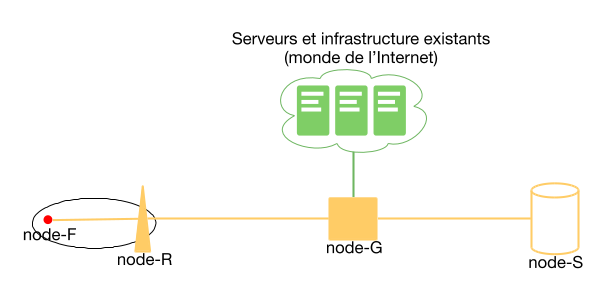
\includegraphics[scale=0.4]{../res/img/archi}
		\caption{Architecture du réseau LoRa FABian}
		\label{fig:archi}
	\end{center}
\end{figure}
\subsection{Mission principale}
La principale tâche réalisée lors de ce stage fut l'amélioration du shield Arduino de la société Wi6Labs. 
Dans un premier temps, j'ai dû nettoyer le code de l'ancienne bibliothèque et dû prendre en main toute la partie Contiki relative au shield.\\
Puis, j'ai dû enlever toute la partie gestion de la MAC et du protocole IEEE 802.15.4 qui était gérée par la carte Arduino pour la programmer à l'intérieur du shield (côté Contiki). J'ai ensuite modifié la partie nommage, c'est-à-dire de pouvoir modifier l'url permettant d'accéder au shield (qui était écrite dans la partie Contiki) depuis internet pour pouvoir le modifier depuis la carte Arduino (en faisant~: \emph{lora.begin("url.s.ackl.io")}).\\
J'ai été chargé de l'amélioration de la gestion de la signalisation. En effet, l'antenne radio envoie des messages de type beacon à la carte Arduino pour lui demander de s'enregistrer. Le problème étant que la carte Arduino ne devait pas recevoir le beacon qui devait être traité seulement dans la partie Contiki.\\
Ce dernier point à mis en valeur la nécessité d'un mode debug sur la carte Arduino pour pouvoir recevoir les messages de type beacon sur la partie Arduino ainsi que la création de méthodes pour pouvoir changer la configuration de la radio (fréquence, coderate, spreading factor, bande passante, etc.), pour plus de flexibilité côté Arduino (et pour éviter de devoir flasher à chaque fois le shield).\\
Finalement, pour rendre le code côté contiki plus propre, j'ai dû modifier le driver radio en place pour pouvoir utiliser la network stack standard\footnote{\url{http://anrg.usc.edu/contiki/index.php/Network_Stack}} qui n'était pas utilisée.\\

\begin{figure}[h]
	\begin{center}
		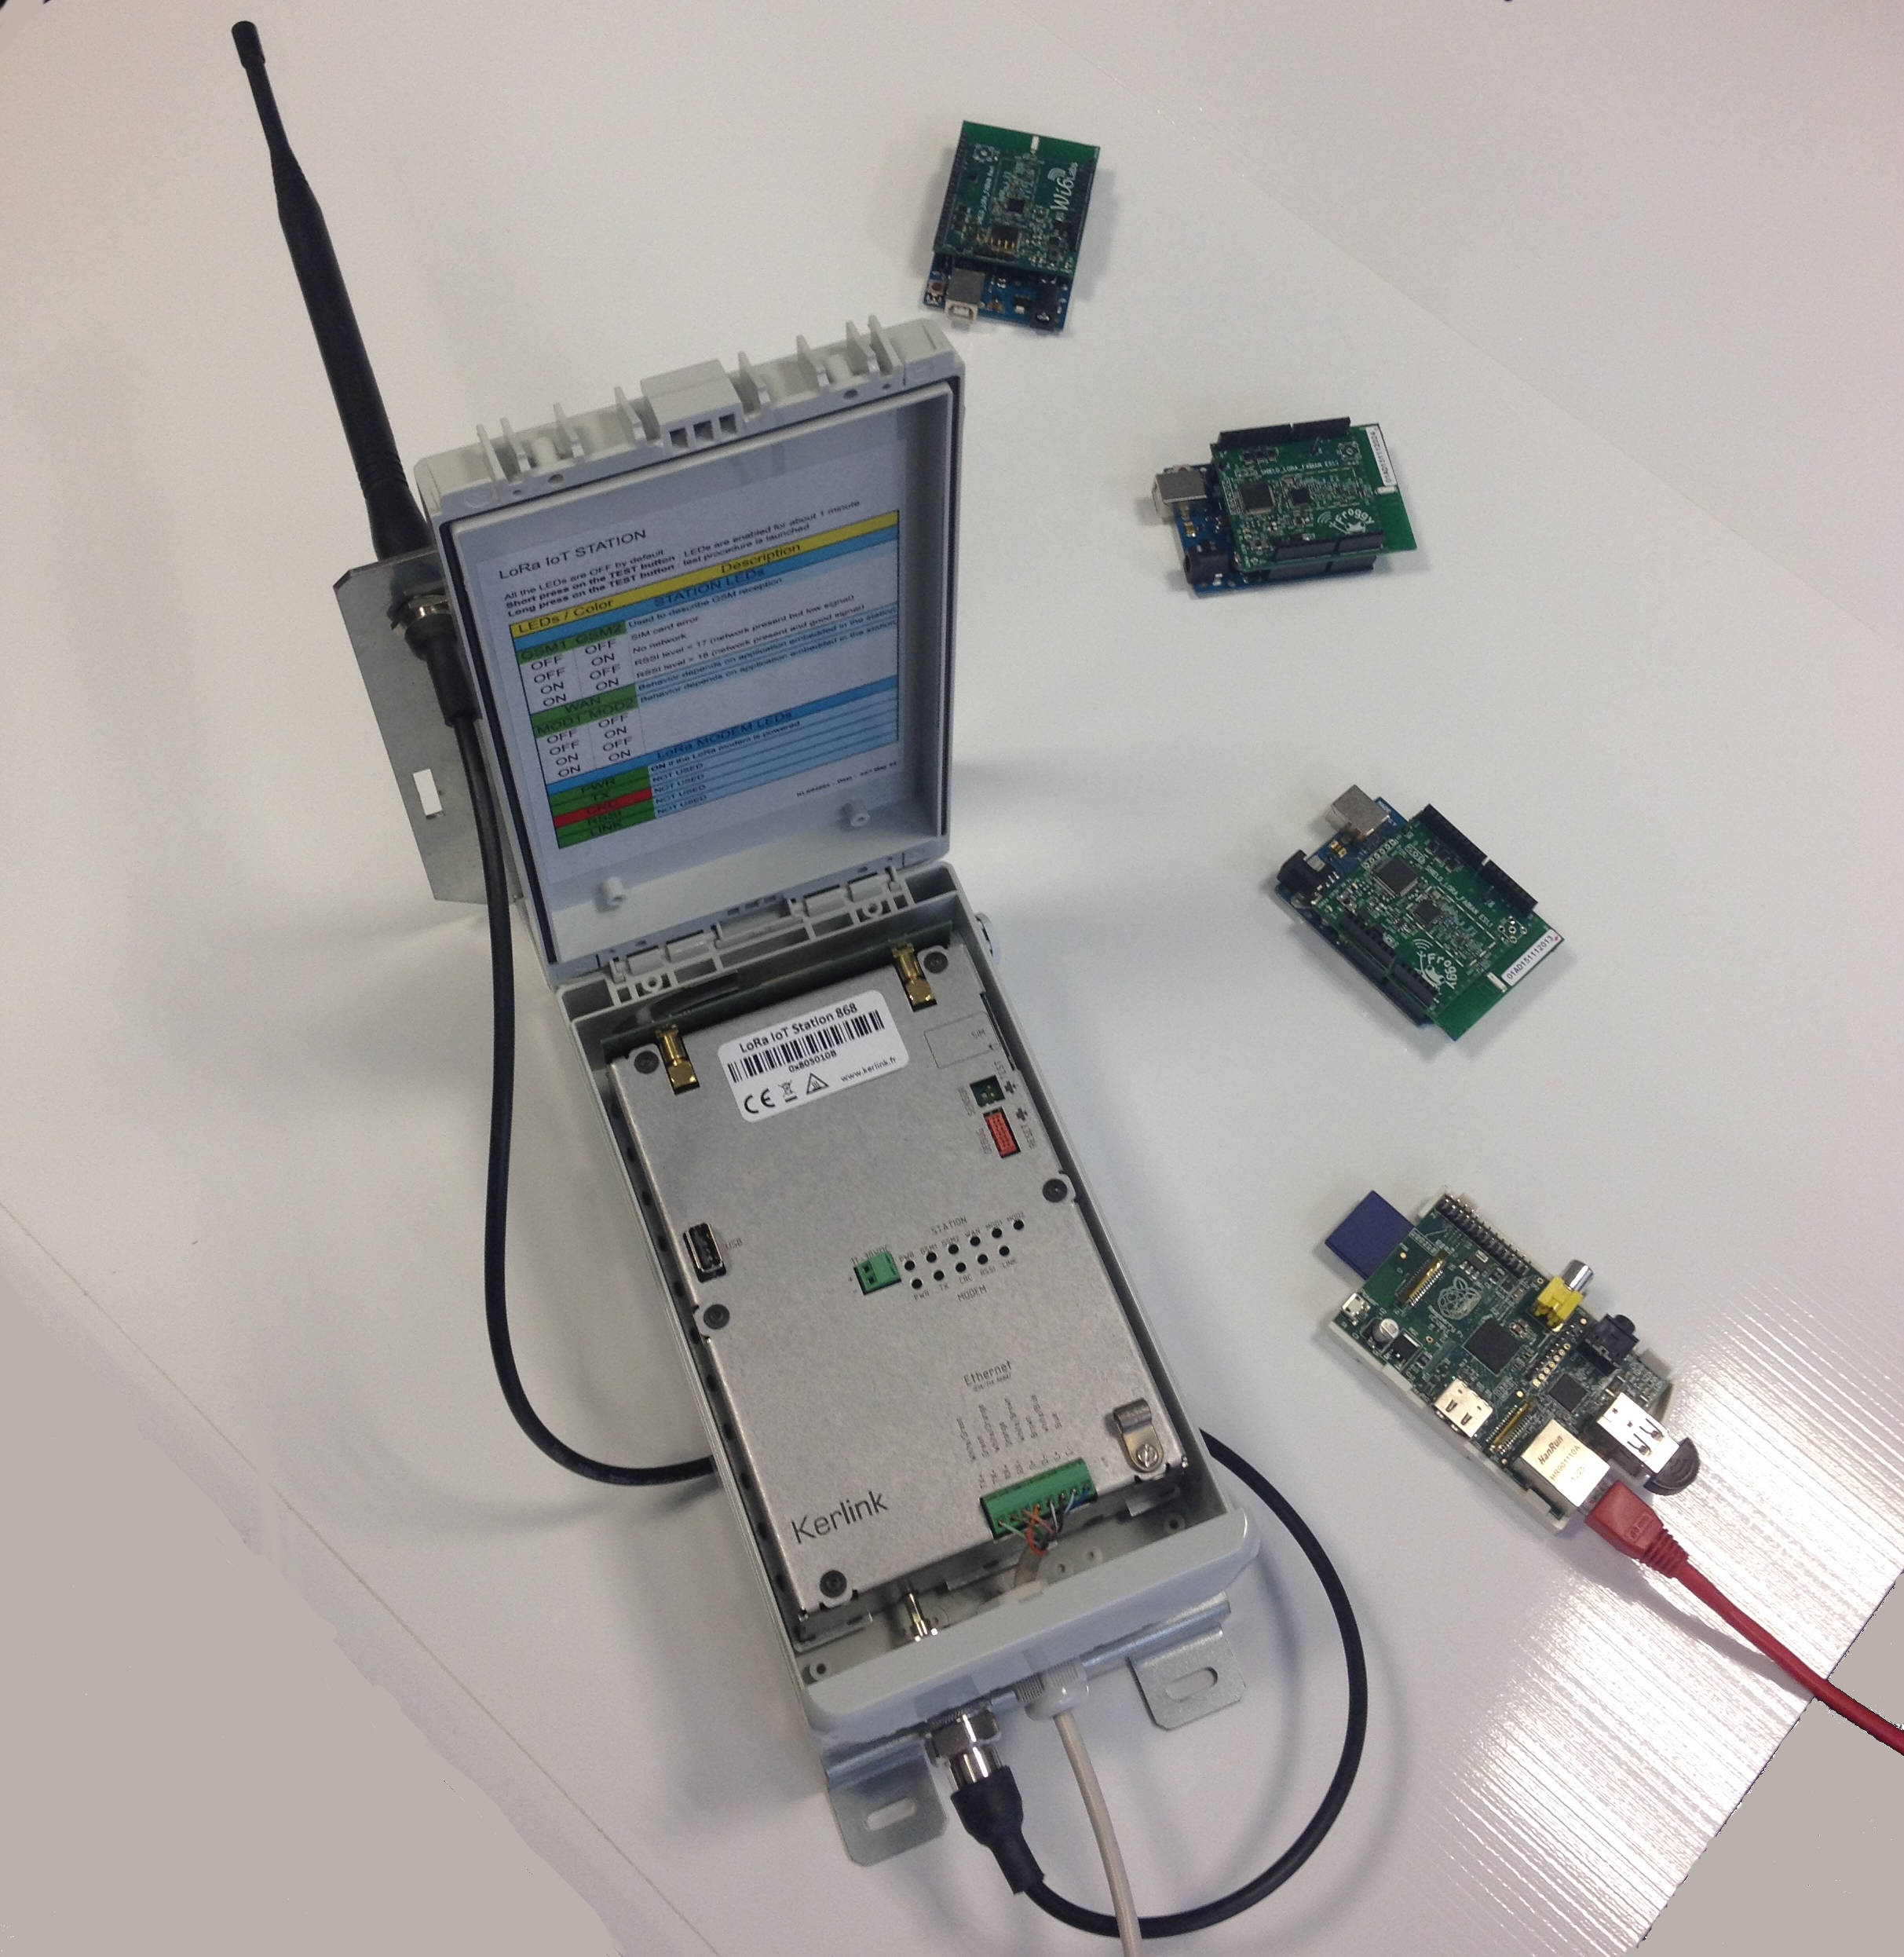
\includegraphics[scale=0.09]{../res/img/antennaNodeF}
		\caption{Une antenne et des noeuds F}
		\label{fig:matoslora}
	\end{center}
\end{figure}

Lors du dernier mois de mon stage, on j'ai travaillé sur le code JAVA qui gérait le node G, c’est-à-dire au niveau de la gateway (sur les projets loraFabian.core et loraFabian.nodeG). Mon but était de mettre en place la partie persistance\footnote{c'est-à-dire de réaliser un mapping objet-relationnel (ORM), ce qui donne un effet de base de données orientée objet (les informations sont stockées sous forme de collections d'objets.)} (sur un environnement MySQL et H2\footnote{Une base de donnée SQL en JAVA - \url{http://www.h2database.com/html/main.html}} ) ainsi que de revoir un peu l’architecture du code et de le documenter. J’ai donc dû prendre en main MAVEN\footnote{automatisation de l'installation des dépendances, de la compilation, de la construction de la documentation - \url{https://maven.apache.org/}}, la JPA\footnote{JAVA Persistence API - \url{http://www.oracle.com/technetwork/java/javaee/tech/persistence-jsp-140049.html}}, eclipselink\footnote{\url{https://www.eclipse.org/eclipselink/}} ainsi que H2. La principale difficulté de cette partie était de travailler avec trois versions de code différentes (la version sur le dépot git, celle du précédent stagiaire qui n’était pas à jour et la mienne).
\subsection{Missions annexes}
J'ai été amené, durant la durée de ce stage à réaliser des missions annexes au projet.\\
Le Week-end du 13 \& 14 Juin, j'ai notamment été co-intervenant devant un public d'une trentaine de personnes lors de la conférence \emph{LoRa FABian~:  projet visant à fournir des protocoles ouverts et standardisés pour les besoins de communication des objets communiquant (IoT)} avec Mathieu \textsc{Goessens} durant l'évènement \emph{Portes Ouvertes Ou Pas} à Paris (Voir annexe A).\\
Le Mercredi 8 Juillet, j'ai aidé à mettre en place la démonstration du projet LoRa FABian lors des Matinales de Rennes Atalante à l'\textsc{INRIA} de Rennes (Voir annexe B). La démonstration consistait à afficher sur une page web (envoyée par la carte Arduino via radio) la valeur d'un capteur de température ou de pouvoir contrôler une led.\\
\section{Bilan du stage}
Ces trois mois de stage m'ont permis d'acquérir une vision concrète du travail d'ingénieur de recherche au sein d'un laboratoire public.
%Bilan des compétences
Ce stage m'a permis de développer plusieurs compétences.\\
Au niveau technique, j'ai pu découvrir quelques protocoles (notamment IEEE 802.15.4 ou CoAP) ainsi que l'environnement Contiki qui m'était totalement inconnu et le shield LoRa de la société Wi6Labs. J'ai pu améliorer mes connaissances en C, python et JAVA (MAVEN, JPA) avec le code réalisé durant ces 3 mois et dans l'environnement Arduino.\\
J'ai eu l'occasion au fil des missions annexes et de la mission principale de travailler en autonomie sur ma mission et de travailler en équipe (notamment pour les missions annexes ou pour les tests).\\
Je me suis aussi trouvé en parfaite autonomie au niveau de mes horaires. En effet, aucun horaire n'était fixé. Lorsque je le pouvais, je commençais tôt le matin avec une veille informationnelle. Ensuite, je programmais ce dont j'avais besoin le matin. L'après-midi étant souvent composée d'une phase de test + debug du code. Enfin je finissais ma journée par de la lecture de documentation et en préparant une TODO list pour les jours suivants.\\
Les missions annexes m'ont aussi permis de développer des compétences. En effet, j'ai pu contribuer à l'organisation de TPs pour des cours d'été (relecture du sujet, programmation des bibliothèques, préparation des cartes, tests en salle) ainsi qu'à la réalisation d'une conférence (modification du diaporama déjà existant, répartition du temps de parole, préparation du texte, présentation devant un public puis réponses à ses questions).\\
%Futur
Ce stage m'a permis de me donner une idée de ce qu'était le travail en laboratoire et dans l'embarqué. Lors de mon prochain stage, je souhaite découvrir le travail dans le Machine Learning et de pouvoir me donner une idée de ce qu'est le travail dans une grande entreprise.
%%%%%%%%%%%%%%%%%%%%%%%%%%%%%%%%%%%%%%%%%%%%%%%%%%%%%%%%%%%%%%%%%%%%%%%%%%%%%%%%%%%%%%%%%%%%%%%%%%%%%%%%%%%%%%%%%
\newpage
\appendix
	\section{Conférence~: Portes Ouvertes Ou Pas}
L'évènement \emph{Portes Ouvertes Ou Pas} s'est déroulé à Paris (20 rue de Reuilly) le 13 \& 14 Juin 2015.\\
Cet évènement est un festival regroupant les collectifs du LOOP (\url{https://wiki.leloop.org/index.php/Wiki.leloop.org}), de la GareXP (\url{http://garexp.org/}) et du Jardin d'Alice (\url{http://www.lejardindalice.org/}).\\
Texte de présentation de la conférence~:\\
\textbf{Lora FABian}\\
    Lora FABian, projet visant à fournir des protocoles ouverts et standardisés pour les besoins de communication des objets communiquant\footnote{Un objet qui communique des informations à un autre objet.} (IoT). On aime ou on aime pas l'IoT, mais si il doit arriver dans nos vies, et vue la durée de vie des objets, autant que ce soit avec des protocoles, implémentations, ouvertes, libres, standardisées, sécurisées.\\
    Plus concrètement, le projet LoRa FABian vise à offrir une stack réseau complète basée sur LoRa (radio longue portée ; très bas débit ; avec pertes) pour exposer des objets vers/depuis internet et masquer toute la complexité de la gestion de réseau. Les objets (typiquement des arduino) parlent en CoAP et sont exposés sur internet en HTTP.\\
Le programme complet est disponible sur le site de l'évènement \url{http://poop.leloop.org/}.\\
Les slides et la vidéo ne sont pas encore disponibles.
	\section{Conférence~: Les matinales de Rennes Atalante}
Le 8 Juillet 2015, l'évènement Matinale Rennes Atalante sur les Smart Cities a eu lieu à l'\textsc{INRIA} de Rennes.\\
Dans le cadre de cette Matinale, nous avons réalisé une démonstration du projet LoRa FABian. La démonstration consistait à répondre à des requêtes CoAP avec des pages web. Par exemple une requête GET sur "beta.s.ackl.io/light" renvoyait une page web montrant la valeur d'un capteur de lumière ainsi qu'une image et un CSS différent en fonction de cette valeur (par exemple, une valeur faible affichait une image de lune sur fond noir).\\
Annonce de l'évènement~: \url{http://www.rennes-atalante.fr/actualites-technopole/agenda-technopole/evenement/prochaine-matinale-smart-city-opportunites-pour-les-entreprises-et-le-territoire.html}
	\section{Travail réalisé}
	Une partie du travail a été réalisée sur un dépot git privé.\\
	Une partie du code a été envoyée sur le git de la société Wi6Labs \url{https://github.com/Wi6labs/lorafabian} ou son fork \url{https://github.com/AmarOk1412/lorafabian}.\\
	Enfin, voici un des TP réalisé~:\\
	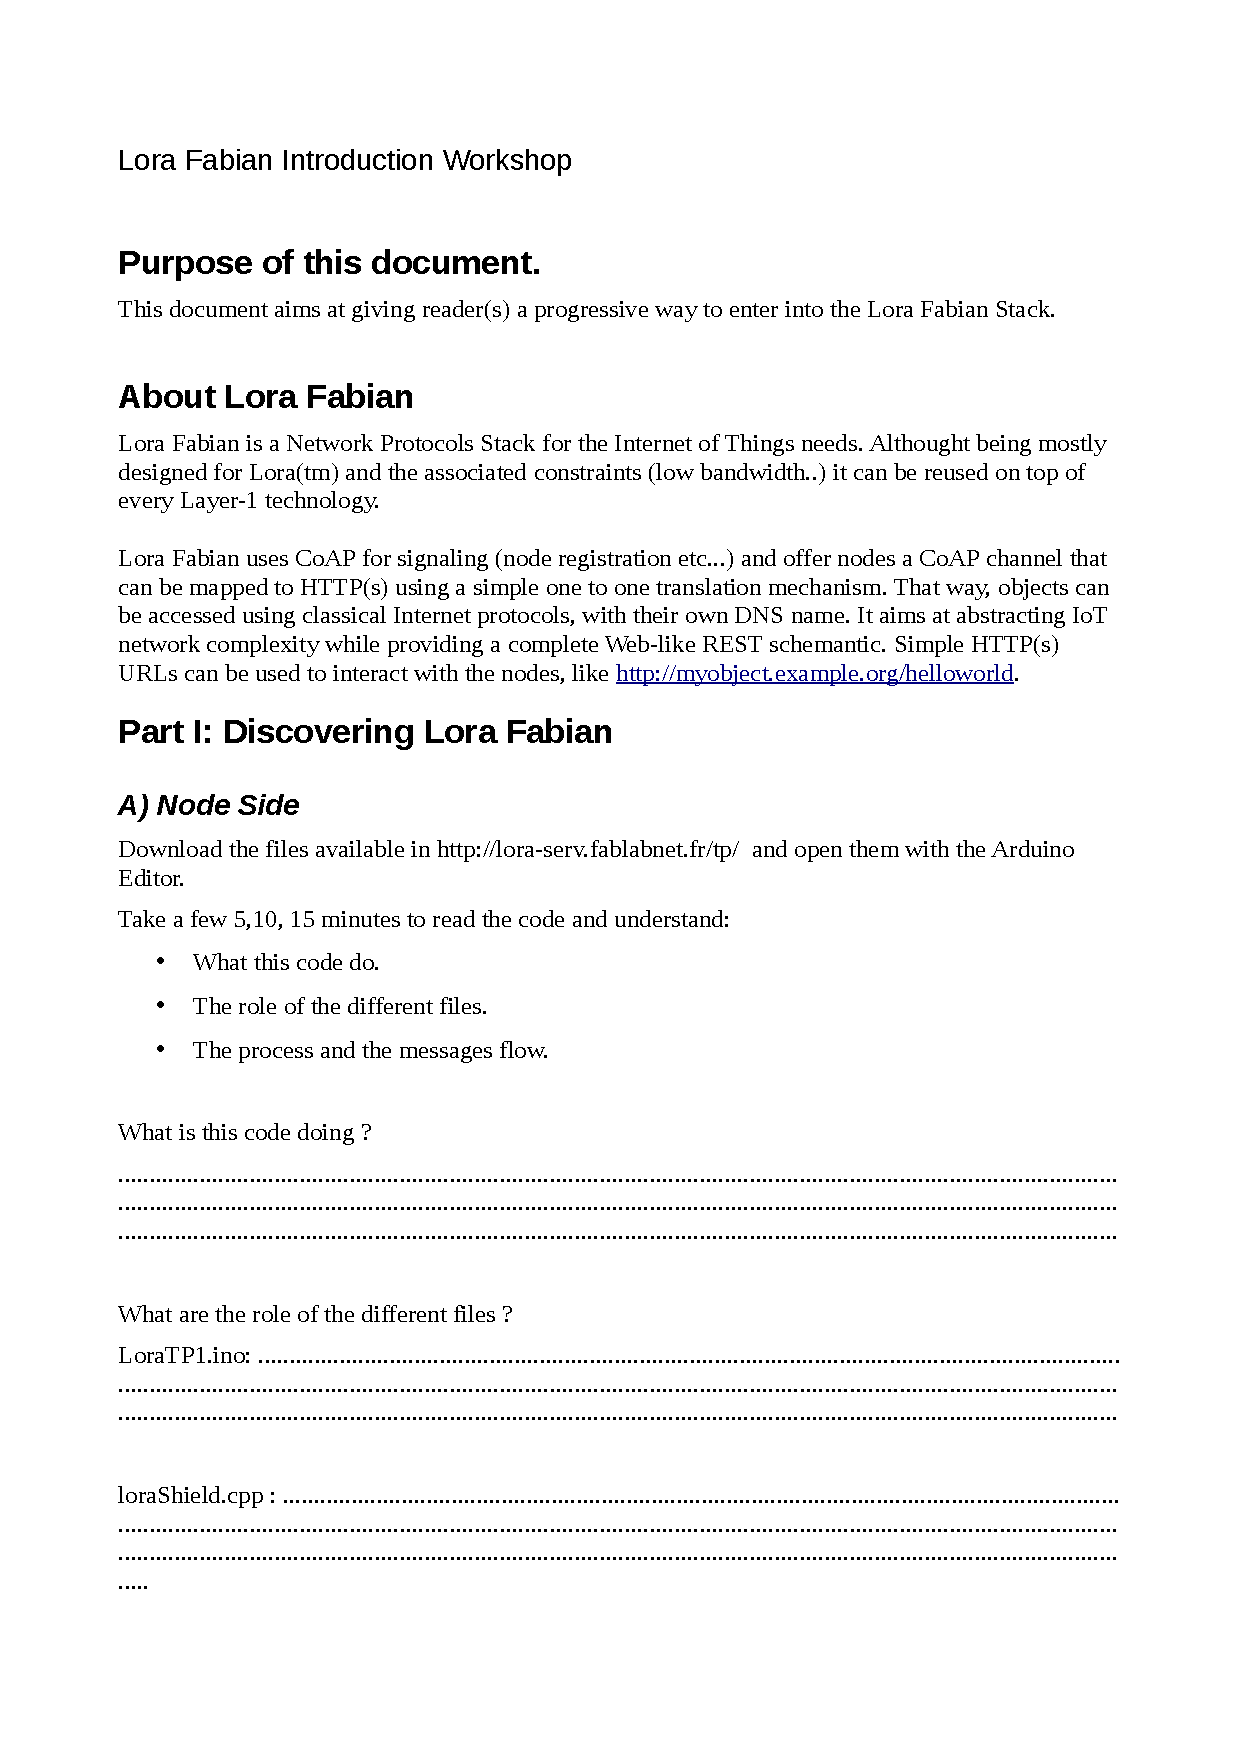
\includepdf[pages={1-5}]{../res/TP-LORA1.pdf}
\end{document}

